\subsection{Input Variables} \label{subsec:vars}
Various sets of per track variables have been explores as inputs to the RNN. These include:
\begin{itemize}
\item Signed transverse and longitudinal impact parameter significance, $S_{d_0}$ and $S_{z_0}$.  Alternatively, the impact parameters, $d_0$ and $z_0$, as well as their errors,  $\sigma(d_0)$ and $\sigma(z_0)$, have been examined as inputs rather than significances.
\item Fraction of jet $p_T$ carried by the track $p_T^{frac} = p_T^{track} / p_T^{jet}$
\item Distance between track and jet axis, $\Delta R(track,\ jet)$. Alternatively, the $\Delta \phi$ and $\Delta \eta$ between the jet and the track have been examined instead of the $\Delta R$
\item The ``track grade", the grading of the track quality as done for IP3D~\cite{IP3D}
\item The number of hits and holes in the silicon detectors has been studied instead of the track grade. Specifically, the variables used were the set \{expectBLayerHit, nBLHits, nInnHits, nNextToInnHits, nPixHits, nSCTHits, nsharedBLHits, nsharedPixHits, nsharedSCTHits, nsplitBLHits, nsplitPixHits \}.
\end{itemize}
Different combinations of these variables were used in the optimization of the performance, as will be seen in Section~\ref{subsec:perfcomp}.

As the tracks in a jet have no intrinsic ordering, several physics inspired orderings were examined: $|S_{d_0}|$, $\sqrt{S_{d_0}^2 + S_{z_0}^2}$, $p_T$.

The baseline training examined here includes the variables: $S_{d_0}$, $S_{z_0}$, $p_T^{frac}$, $\Delta R(track,\ jet)$, and track grade. Tracks are ordered by $|S_{d_0}|$.


\subsection{Architectures} \label{subsec:arch}
Several RNN based architectures were examined. For each network, after the RNN layer(s), the last time step output was fed into a dense layer, followed by a logistic regression layer for classification.
\begin{itemize}
\item In the case of using the track grade, a categorical variable, a linear embedding was used to map categories into continues vectors.  The default embedded vector size was 2, but other sizes were examined. In the case of hits, not embedding was needed.
\item Single layer of LSTM units, or two stacked on top of each other.
\item Using LSTM units versus using gated recurrent units (GRU)~\cite{GRU}.
\item 2 class output ($b$ vs. not $b$), and 4 class output ($b$, $c$, light, $\tau$).
\end{itemize}


\subsection{Performance Comparisons} \label{subsec:perfcomp}
To understand the performance and the convergence of the recurrent neural network, we cross-check the performance of the nominal network with many different neural network configurations as well as variations of input. 

The number of RNN layers as well as the number of nodes in each RNN layer are the basic parameters of RNN models and could affect the peformance of RNN based IP tagger. We vary these two parameters by setting number of nodes to 25 and 50 and number of layers to 1 and 2. In general, we find 2-layer and 1-layer RNNs show similar performance while models with 50 nodes outperform those with 25 nodes as shown in Figure ~\ref{fig:LayersAndNodes}. 

Recurrent neural networks are known to be slowly converging. We vary the number of trainning epochs from 40 to 100 to check if the training is fully converged and the weights of the network are stable. The RNNs trained with different number of epochs show negligible difference in performance as presented in Figure ~\ref{fig:Epochs}. 

Increasing the depth of the neural network could potentially improve the performance of a classifier. In the case of RNN based IP tagger, we explored the variation of adding one more dense layer right before the output layer. As shown in Figure ~\ref{fig:MoreDense}, such variation does not yield significant gain in performance..

The effect of information of inputs at early time stamps get diluted at later time-stamps is called vanishing gradient, which is a known generic problem for RNN. Cells liks LSTM help to alleviate the problem but does not gaurantee randomly ordered track sequences would have the same performance. We compare the nominal physics motivated track ordering, tracks ordered in decreasing $|S_{d0}|$ values, to other orderings including: decreasing track $|S_{L0} = \sqrt{S_{d0}^2+S_{z0}^2}|$ ordering and increasing track $|S_{d0}|$ ordering. We do not observe significant performance difference with different track orderings as shown in Figure ~\ref{fig:Ordering}. 

The simulated $t\bar t$ events have 10\% $c$-jets. Historically we observed in the training of other taggers that varying the amount of $c$-jets in the training sample would affect the performance. We check this effect by reducing the fraction of $c$-jets to 5\% and find the RNN is insensitive to this amount of jet flavor fraction change as shown in Figure ~\ref{fig:CFrac}.

Gated Recurrent Unit (GRU, reference) is a more recent and simplified version of RNN cell compared to LSTM. We experimented to construct RNNs with GRU cell while fixing other model and training parameters. As shown in Figure ~\ref{fig:GRU}, GRU based RNN has similar performance as LSTM based RNN network. 

The underlying $p_{T}$ distributions of $b$, $c$ and light jets are different. We know that the b-tagging performance is highly $p_{T}$ dependent. If a particular analysis targets phase space which is significantly different from the training sample, i.e. $t\bar t$ events, we need to train taggers with same underlying $p_{T}$ distributions for each flavor. As shown in Figure ~\ref{fig:pTReweight}, re-weighting $b$ and $c$ jets $p_{T}$ distributions to that of light jets decreases the RNN tagger performance as expected. However it is worth nothing that the RNN taggers are still significantly better than baseline taggers like SV1 and IP3D.


\begin{figure}[htbp]
  \centering
 \includegraphics[width=0.48\textwidth]{figures/ModelVariations/ROC_LSTM_2nLayer_BL.png}
 \includegraphics[width=0.48\textwidth]{figures/ModelVariations/ROC_LSTM_2nLayer_BC.png}
 \includegraphics[width=0.48\textwidth]{figures/ModelVariations/ROC_LSTM_2nLayer_4Class_BL.png}
 \includegraphics[width=0.48\textwidth]{figures/ModelVariations/ROC_LSTM_2nLayer_4Class_BC.png}

\caption{ROC curves of RNN built with different number of recurrent layers and different number of nodes in each layer}
  \label{fig:LayersAndNodes}
\end{figure}

\begin{figure}[htbp]
  \centering
 \includegraphics[width=0.48\textwidth]{figures/ModelVariations/ROC_LSTM_Epoch_BL.png}
 \includegraphics[width=0.48\textwidth]{figures/ModelVariations/ROC_LSTM_Epoch_BC.png}
 \includegraphics[width=0.48\textwidth]{figures/ModelVariations/ROC_LSTM_Epoch_4Class_BL.png}
 \includegraphics[width=0.48\textwidth]{figures/ModelVariations/ROC_LSTM_Epoch_4Class_BC.png}

\caption{ROC curves of RNN trained with different number of epochs}
  \label{fig:Epochs}
\end{figure}


\begin{figure}[htbp]
  \centering
 \includegraphics[width=0.48\textwidth]{figures/ModelVariations/ROC_LSTM_MoreDense_BL.png}
 \includegraphics[width=0.48\textwidth]{figures/ModelVariations/ROC_LSTM_MoreDense_BC.png}
 \includegraphics[width=0.48\textwidth]{figures/ModelVariations/ROC_LSTM_MoreDense_4Class_BL.png}
 \includegraphics[width=0.48\textwidth]{figures/ModelVariations/ROC_LSTM_MoreDense_4Class_BC.png}

\caption{ROC curves of RNN trained with different number of epochs}
  \label{fig:MoreDense}
\end{figure}


\begin{figure}[htbp]
  \centering
 \includegraphics[width=0.48\textwidth]{figures/ModelVariations/ROC_LSTM_Order_BL.png}
 \includegraphics[width=0.48\textwidth]{figures/ModelVariations/ROC_LSTM_Order_BC.png}
 \includegraphics[width=0.48\textwidth]{figures/ModelVariations/ROC_LSTM_Order_4Class_BL.png}
 \includegraphics[width=0.48\textwidth]{figures/ModelVariations/ROC_LSTM_Order_4Class_BC.png}

\caption{ROC curves of RNN trained with differently ordered track sequences}
  \label{fig:Ordering}
\end{figure}

\begin{figure}[htbp]
  \centering
 \includegraphics[width=0.48\textwidth]{figures/ModelVariations/ROC_LSTM_LessC_BL.png}
 \includegraphics[width=0.48\textwidth]{figures/ModelVariations/ROC_LSTM_LessC_BC.png}
 \includegraphics[width=0.48\textwidth]{figures/ModelVariations/ROC_LSTM_LessC_4Class_BL.png}
 \includegraphics[width=0.48\textwidth]{figures/ModelVariations/ROC_LSTM_LessC_4Class_BC.png}

\caption{ROC curves of RNN trained with different fractions of $c$-jets}
  \label{fig:CFrac}
\end{figure}


\begin{figure}[htbp]
  \centering
 \includegraphics[width=0.48\textwidth]{figures/ModelVariations/ROC_GRU_BL.png}
 \includegraphics[width=0.48\textwidth]{figures/ModelVariations/ROC_GRU_BC.png}

\caption{ROC curves of RNN built with Gated Recurrent Unit}
  \label{fig:GRU}
\end{figure}


\begin{figure}[htbp]
  \centering
 \includegraphics[width=0.48\textwidth]{figures/ModelVariations/ROC_LSTM_JetpTReweight_BL.png}
 \includegraphics[width=0.48\textwidth]{figures/ModelVariations/ROC_LSTM_JetpTReweight_BC.png}
 \includegraphics[width=0.48\textwidth]{figures/ModelVariations/ROC_LSTM_JetpTReweight_4Class_BL.png}
 \includegraphics[width=0.48\textwidth]{figures/ModelVariations/ROC_LSTM_JetpTReweight_4Class_BC.png}

\caption{ROC curves of RNN trained with re-weighting $b$ and $c$ jets $p_{T}$ to that of light jets}
  \label{fig:pTReweight}
\end{figure}


\clearpage
\subsection{Efficiency and rejection vs. $p_T$}

\begin{figure}[htbp]
  \centering
 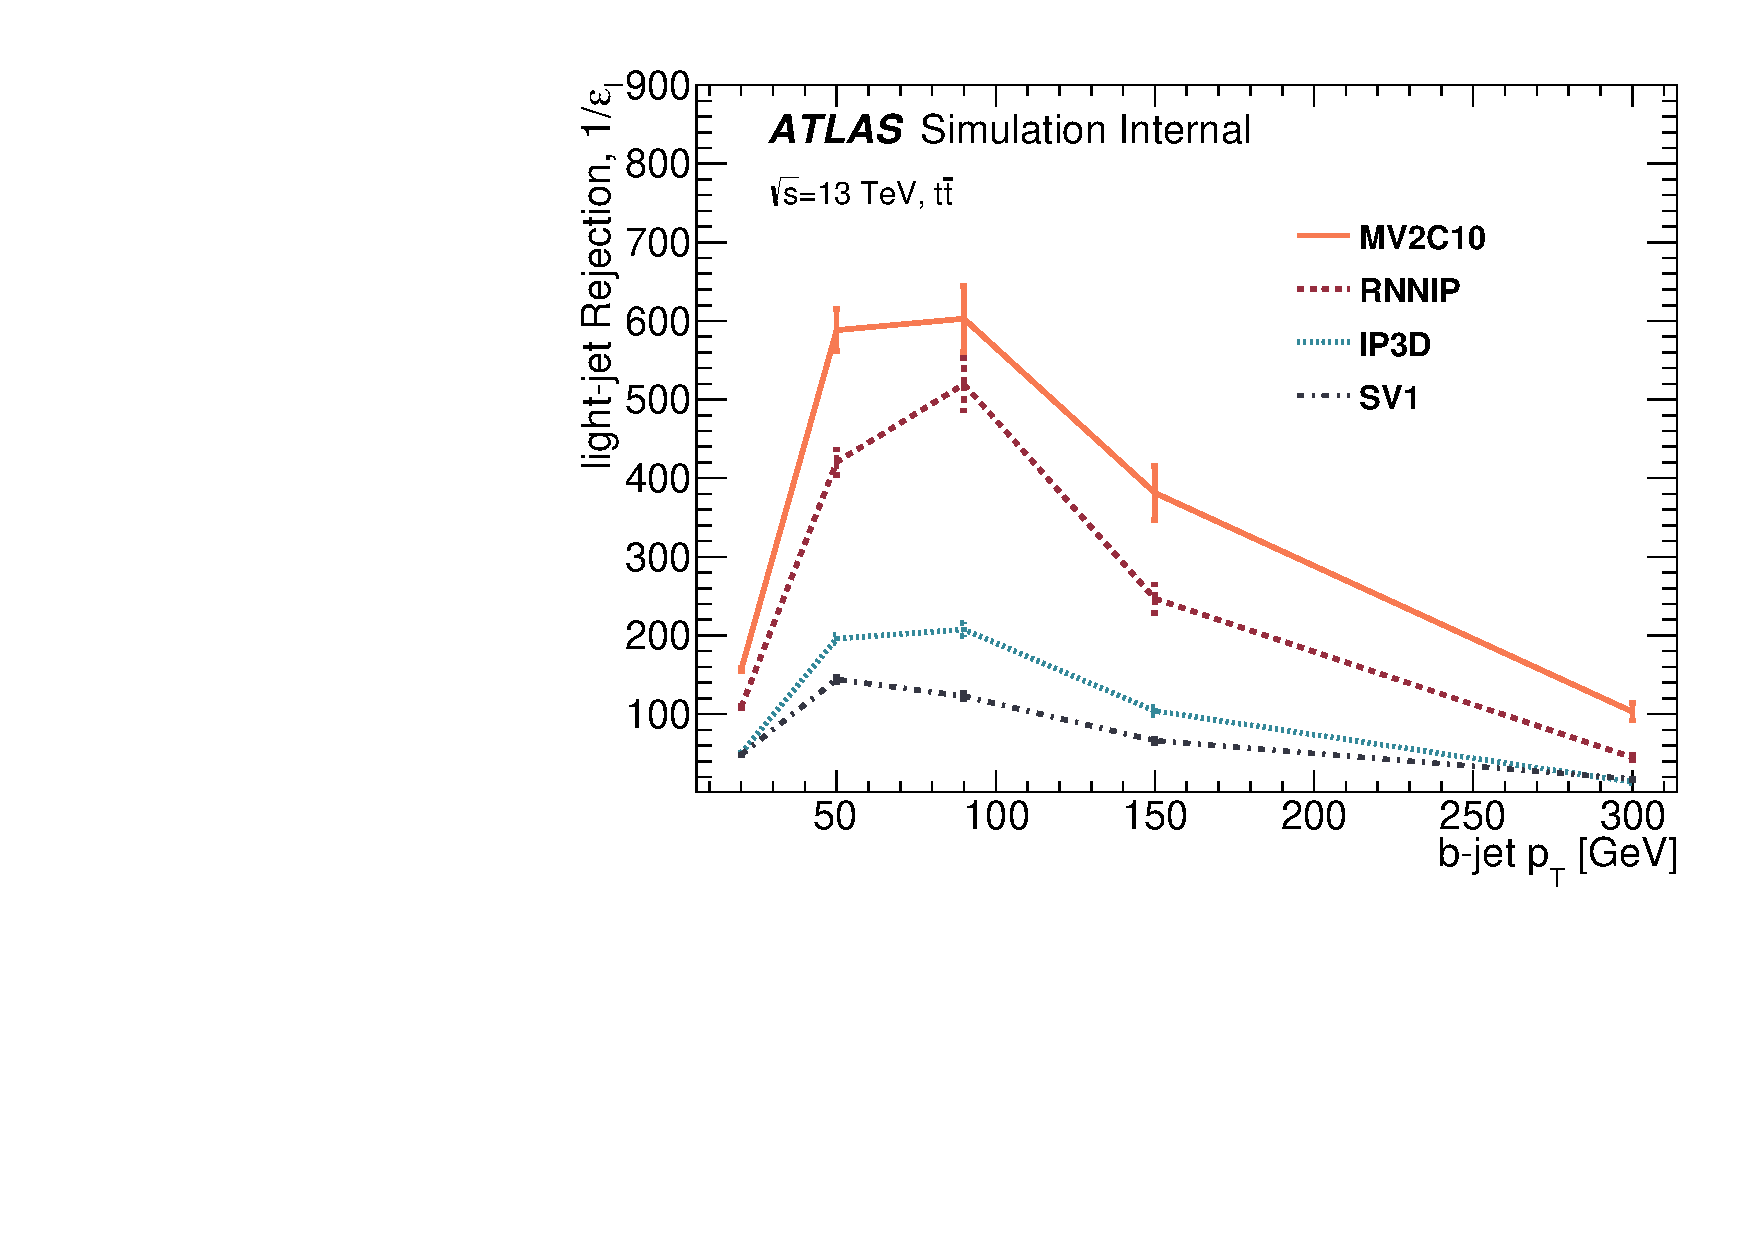
\includegraphics[width=0.48\textwidth]{figures/Perf/LRej_FlatEff.png}
\caption{Light jet rejection at flat b-tagging efficiency of 70\% versus jet $p_T$.}
  \label{fig:LRej_flat}
\end{figure}

\begin{figure}[htbp]
  \centering
 \includegraphics[width=0.48\textwidth]{figures/Perf/BEff_FixedWP.png}
 \includegraphics[width=0.48\textwidth]{figures/Perf/LRej_FixedWP.png}

\caption{$b$-tagging efficiency (left) and Light jet rejection (right) for a fixed 70\% WP cut versus jet $p_T$. }
  \label{fig:input_output_corrs}
\end{figure}



\clearpage
\subsection{Correlations}

\begin{figure}[htbp]
  \centering
 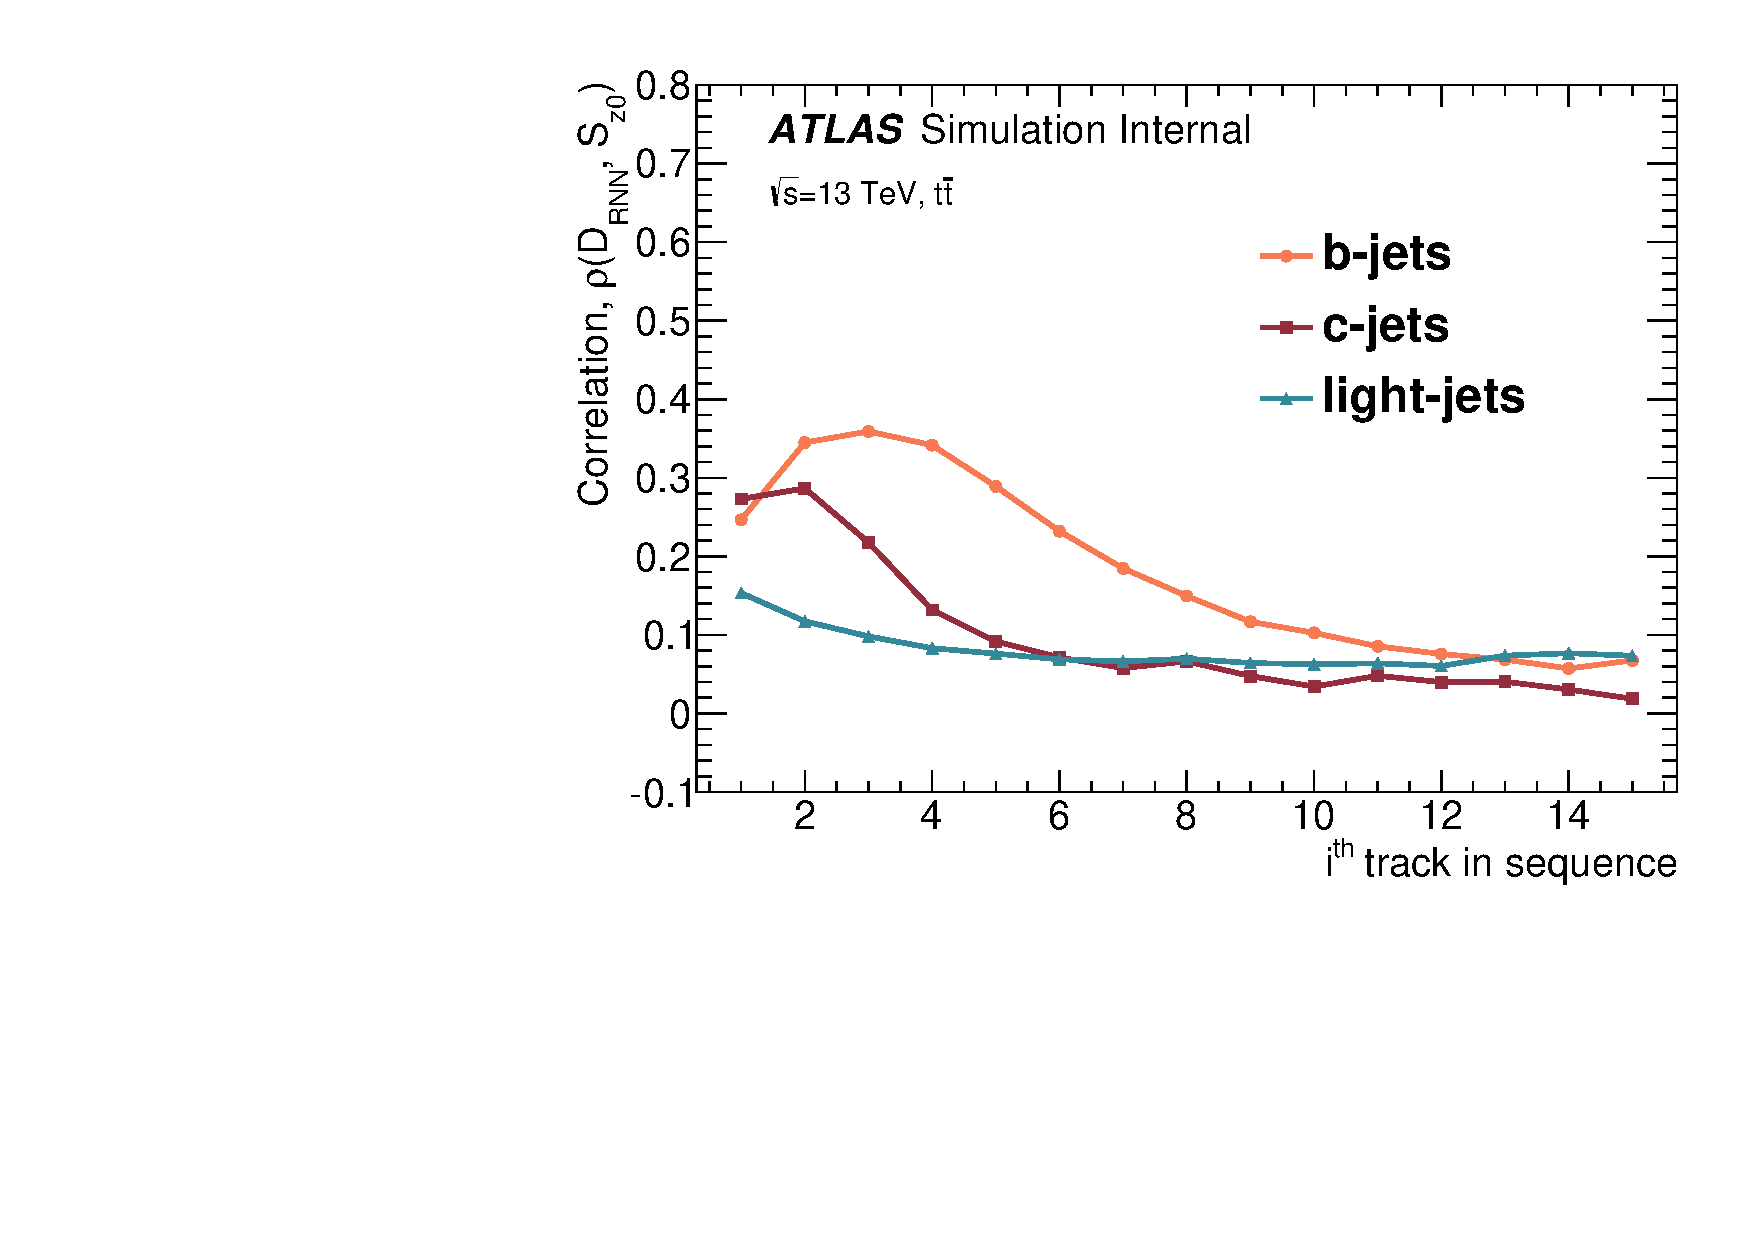
\includegraphics[width=0.48\textwidth]{figures/Perf/Corr_Sz0.png}
 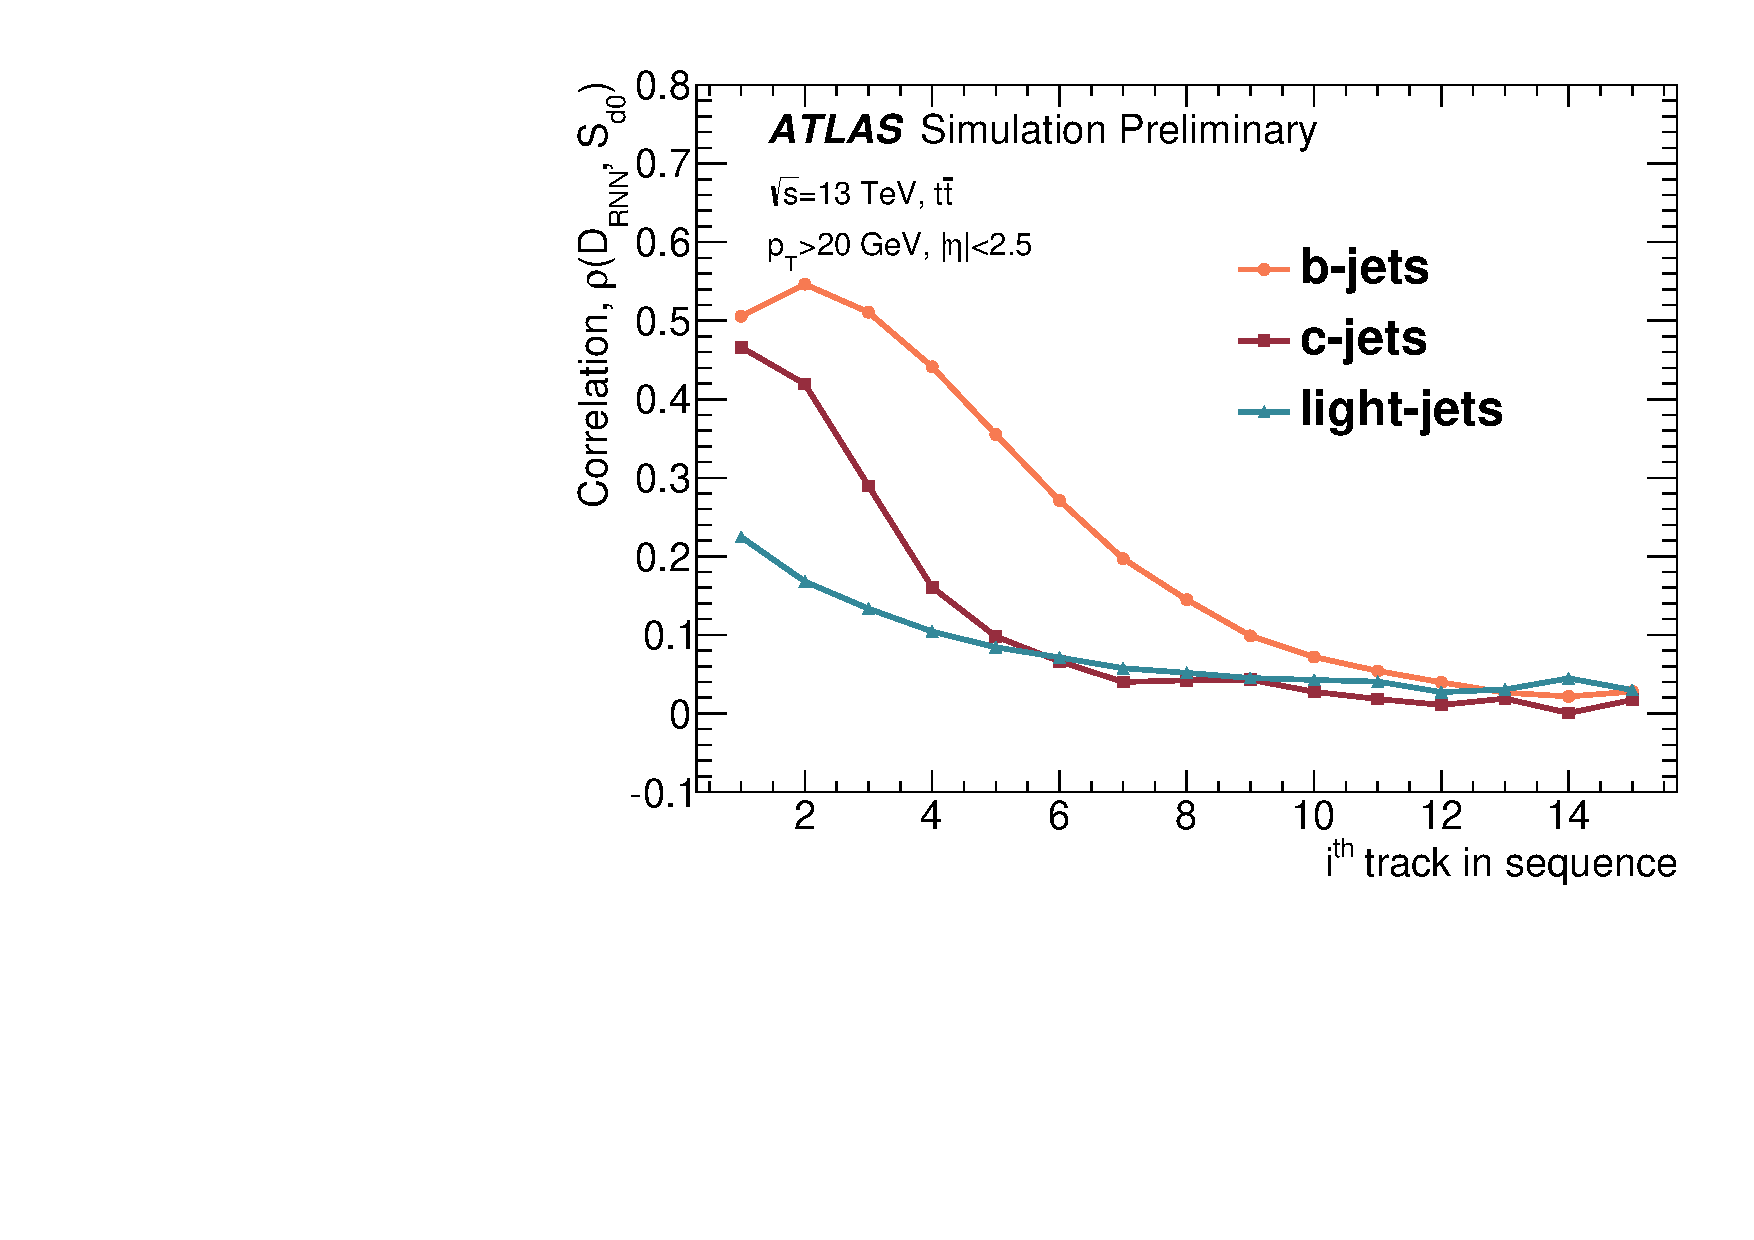
\includegraphics[width=0.48\textwidth]{figures/Perf/Corr_Sd0.png}
 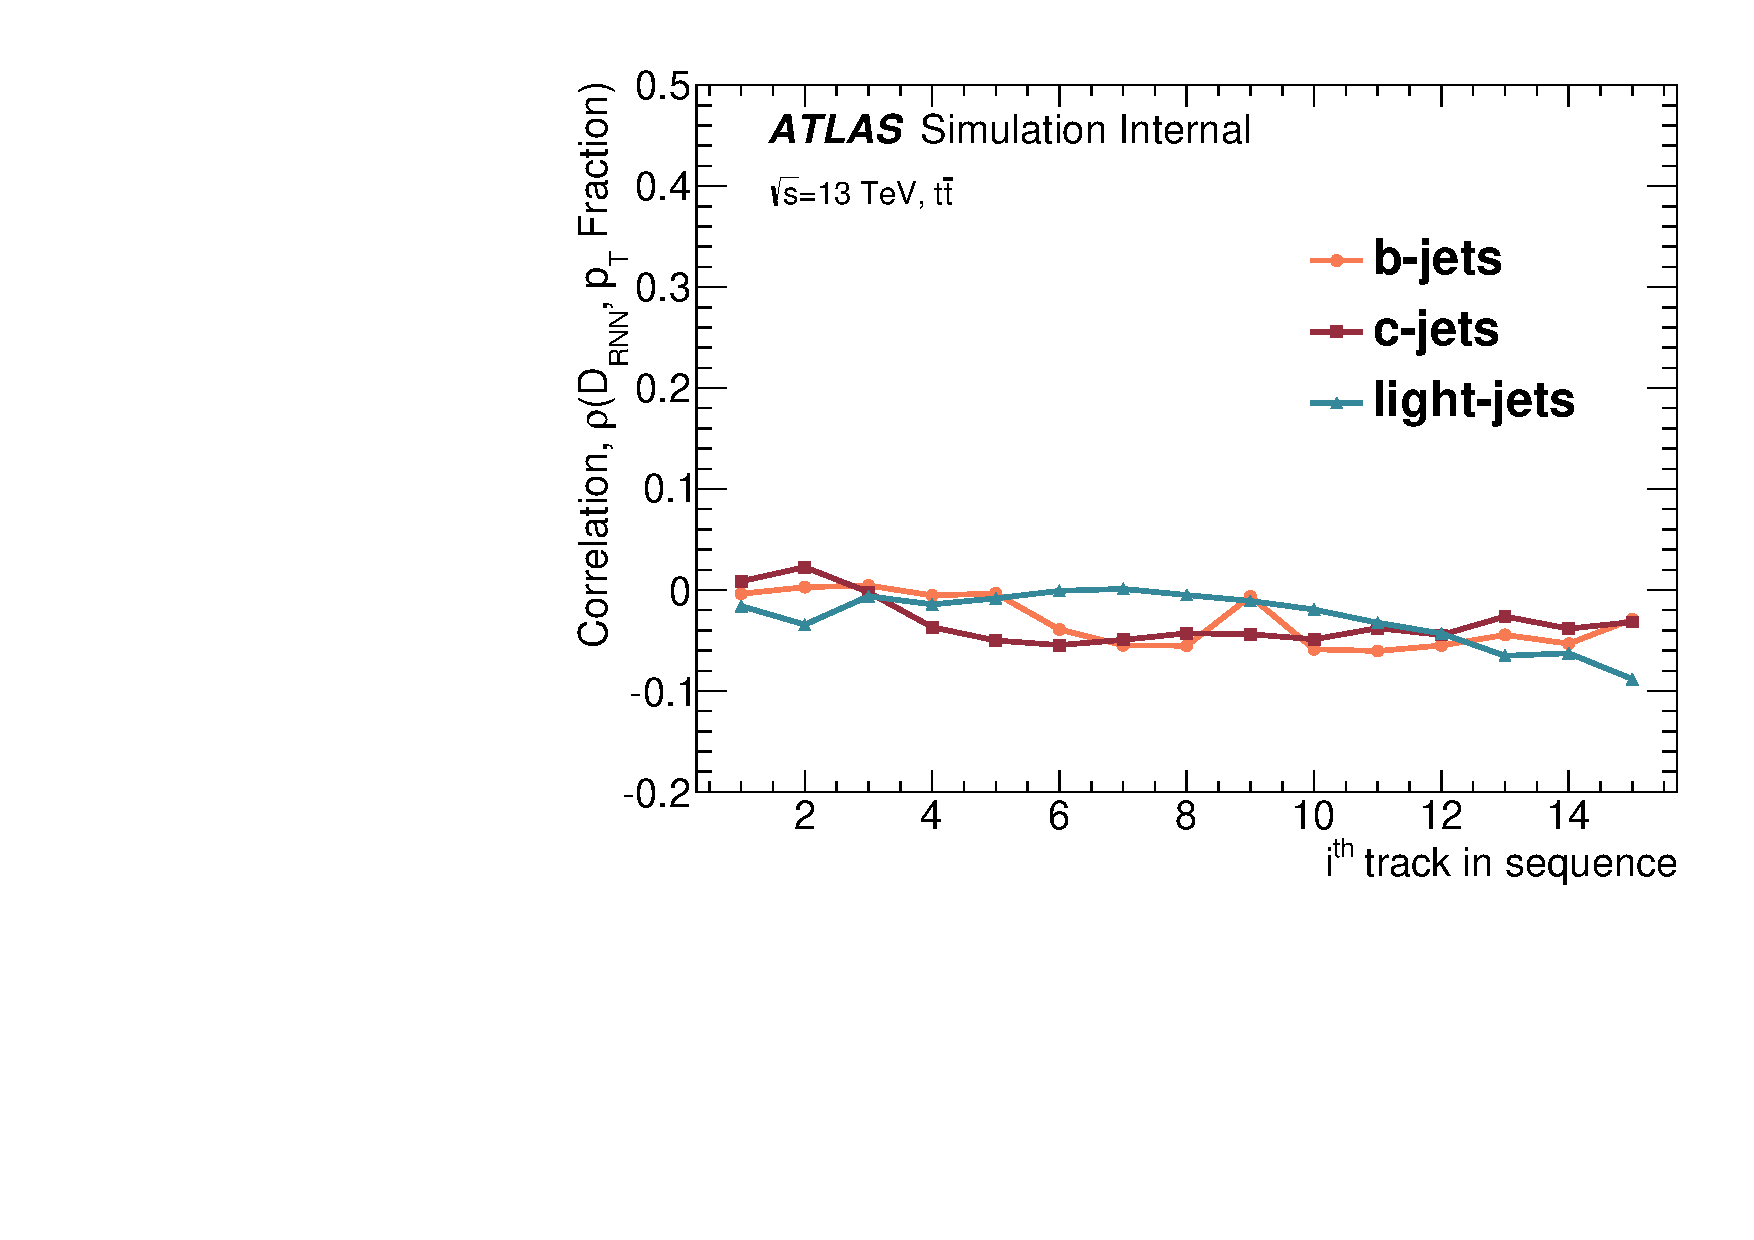
\includegraphics[width=0.48\textwidth]{figures/Perf/Corr_pTFrac.png}
 \includegraphics[width=0.48\textwidth]{figures/Perf/Corr_dR.png}

\caption{Correlations of per track input variables with the RNN output.}
  \label{fig:input_output_corrs}
\end{figure}
